\hsection{The Database Lifecycle}%
The design of \dbs\ is not a straightforward process of \inQuotes{idea $\rightarrow$ design $\rightarrow$ finished.}
Instead, designing good \dbs\ involves several steps.
We need to clearly understand the requirements for the \db.
We should create a rough sketch of what things will be included.
We need to decide what tables and relations should exist.
This conceptual schema~(information about the types of data and their relationships) must then be mapped to a physical schema (concrete implementation instructions for a selected~\dbms).
There should be some sort of prototype, where we and the users can enter a subset of the data to test whether everything works as predicted.
At this stage, we may uncover some problems and may need to improve our design.
The actual application must then be tested.
Then, once we are happy with everything, the application and \db\ enter the productive environment.
They need to be maintained and backed up regularly.
Due to the longevity of \dbs, eventually, new features and changes may become necessary, at which point we may need to revise our design.
There exist several general approaches on how to manage or conduct the \db\ design process, how to bring this process into some structure~\cite{GMTM2011DDLC}.

\Pglspl{db} are software artifacts, so we could use one of the many available \pglspl{SDLC}~\cite{I2018SAH,N2024SEFDS}.
Yet, \dbs\ are also special.
They are objects with a comparatively long lifetime~\cite{SS2005EIDDDFDB:I}.
The hardware in your computer stays the same maybe for three to five years.
Software programs often change every five to ten years.
Every two years, a new long term support~(LTS) version of the \ubuntu\ operating system comes out~\cite{C2024TULARC}.
\libreoffice\ releases every six months~\cite{DF2024TDFWR}.
Major versions of \microsoftWindows\ come out every two to six years~\cite{GLRGRLJH2025LOWV}.
Once new major versions of such important software appear, the old versions usually fade out of support within five years and need to be replaced.

\Pglspl{db}, however, may stay in use for several decades.
Indeed, a long time ago, I designed a \db\ that was used by a branch office of a midsized company for well over a decade.
Therefore, \dbs\ and the applications built on top of them are important assets of en organization.
They contain valuable information, both historical data as well as the data required by the current operation.

\Pglspl{db} are not just used to store data, the data they store mirrors real-world entities and processes.
In our small factory example, the data mirrors the products, the customers, and the interactions of the customers with the factory.
Any of them may well change over time.
For example, maybe the company eventually changes from selling products with a fixed name and configuration to configurable products.
Maybe one day a customer can decide the color and size of the shoes they want to order together with the cloth to be used as well as the material of the sole.
This could yield so many possible combinations that the current way to store products is no longer feasible.
Maybe the scope of the \db\ is eventually expanded to also keep track of the product stock in the warehouse.

All of the above together lead to several demands on the \db\ development lifecycle.
This lifecycle is very similar to the software development lifecycle.
It often even is either the backend or the foundation of software development.
However, there are two aspects that make the \db\ development special:
First, the longevity of \dbs.
Second, there is the \inQuotes{low-levelness} of \dbs.
Since the \db\ is the very foundation upon which other applications like reports, forms, and websites are developed, they are the first point of contact between project stakeholders and developers.
The \db\ development process is where the basic understanding of the data and processes in an organization is built.
This is where the situation is most uncertain, where most of the misunderstandings will happen.

The foremost and obvious requirement to the \db\ design process is that it guides us to translate the information from the stakeholders to a fully functional and running \db\ application.
It should allow us to plan how to do the project, i.e., to create a timeline defining when we will reach which milestone, how many work hours may be needed, and how much things are going to cost.

More often than not, the stakeholders are initially not entirely clear about their processes and data.
During the first few discussions about what the \db\ should store and do, several important details may be missed.
For example, \inQuotes{Each product has a name.} seems to be a reasonable statement when designing a \db\ for a factory.
The \db\ designer thus may just assume that this is true and not double-check or discuss this aspect in-depth.
However, sometimes we may be in for a surprise, maybe the following could happen:
\inQuotes{Ah, indeed, we use different product names for different customers. %
This customer, for example, is a big company that uses our screws to build cars. %
When we offer them our \inQuotes{Screw~3B} we call it \inQuotes{double-inch screw,} because this is how they refer to it in their production processes.}
Obviously, such a situation could not be captured with a single table per product anymore.

Also, many real-world processes are not entirely formally specified.
Processes that modify the ata may have a very clear core, e.g., \inQuotes{We send the product to the customer's address once they paid.}
But there might be fuzzy edges, like \inQuotes{Very few of our customers have been with us for many years or buy lots of products, they can pay after receiving the product.}
If we design a \db\ for managing students, it may be that the school says:
\inQuotes{A student can repeat an exam at most twice after failing it.}
In reality, there might be special circumstances under which some students may be granted a third trial, maybe a student arrived late to an exam due to traffic and was marked as failure, but the exam commission decides to given them another chance.
Therefore, problems may be discovered early in the \db\ design process but could just as well be encountered a year after the \db\ application has been deployed.

Sometimes, the customer may also just assume that some things are common knowledge.
\inQuotes{Of course, for customers with a delivery address outside of the European Union, we add an export tax. %
All businesses do that. %
Everybody knows that.}
The \db\ designer may not know that, though.

Therefore, a \db\ design process should also allow us to progressively enhance our design in response to uncovered issues~\cite{GMTM2011DDLC,WK1989DKBSRTSDLC}.
At the same time, it should avoid scope creep, i.e., a situation where progressive enhancements keep modify the project structure, adding more and more features, and drifting away from the originally planned project~\cite{GMTM2011DDLC,WK1989DKBSRTSDLC}.%
%
%
\hsection{Classical Software Engineering Design Processes}%
\FloatBarrier%
%
\begin{figure}%
\centering%
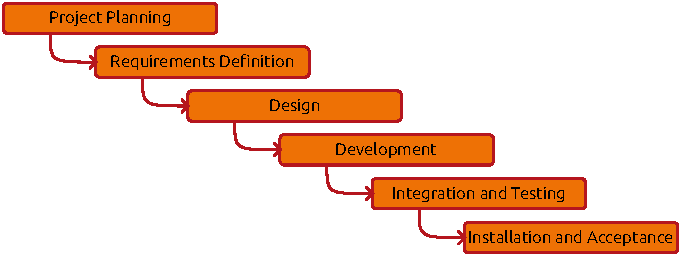
\includegraphics[width=0.8\linewidth]{\currentDir/waterfall}%
\caption{The waterfall model~\cite{PM2020SEAPA,GMTM2011DDLC,I2018SAH,N2024SEFDS}.}%
\label{fig:model:waterfall}%
\end{figure}%
%
Several different design methods, i.e., \pglspl{SDLC}, have been proposed in the field of software engineering.
The simplest is the waterfall model~\cite{PM2020SEAPA,GMTM2011DDLC} illustrated in \cref{fig:model:waterfall}.
The waterfall model is a sequential process of project planning, requirements definition, design, development, testing, and installation and project acceptance.
Each step produces deliverables as output which become the input for the next phase.
During the requirements definition phase, the project scope is restricted based on the discussions with the stakeholders.
The waterfall model specifies which activities should be carried out in each phase as well as the deliverables that should be produces.
The waterfall model is simple and easy to implement.
It allows the developers to work their way along a well-known structure.
At each phase of the project, we know where we are standing and there thus will be few misunderstandings.

However, the model is strictly sequential.
It does not anticipate that there can still be misunderstandings and that we may still discover unexpected issues.
There is no feedback and return to previous phases built-in.
The requirements are specified early in the process and there is no predefined mechanism to introduce changes later in the project.

\begin{figure}%
\centering%
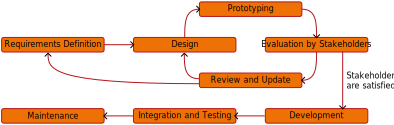
\includegraphics[width=0.8\linewidth]{\currentDir/prototype}%
\caption{The prototyping model~\cite{PA2009SETAP,GMTM2011DDLC}.}%
\label{fig:model:prototype}%
\end{figure}%
%
Another idea is to embrace that both the stakeholders and the developers do not clearly know what the final product should look like and to put a cycle of prototypes and discussions into the center of the development process.
This prototyping process is illustrated in \cref{fig:model:prototype}~\cite{PA2009SETAP,GMTM2011DDLC}.
First, a limited version of the requirements are collected and a prototype of the \db\ and software is designed right away.
The prototype may even be a mockup which only shows the basic functionality of the project and does not interact with other tools.
It serves as basis for discussions and may need to be redesigned.
The final product may look different from the prototype, which creates some uncertainty.
The prototyping model provides the ability of iterative enhancement of the project specification, but sacrifices some clarity of process sequence.
In the prototyping model, the requirements are still finalized early on.
The iterative part is focused on the design, prototyping, evaluation by the stakeholders, and reviews.

\begin{figure}%
\centering%
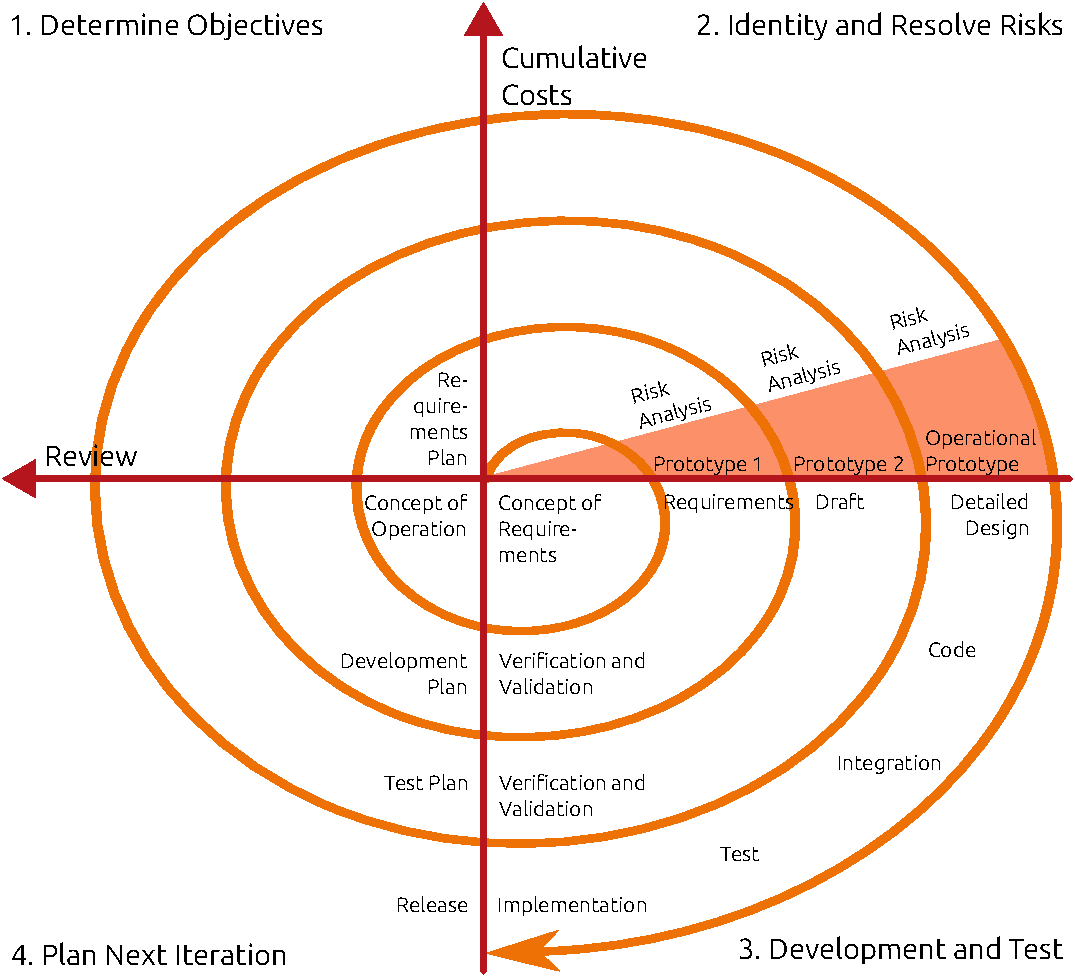
\includegraphics[width=0.8\linewidth]{\currentDir/spiral}%
\caption{The spiral model~\cite{S2007OOSE,GMTM2011DDLC}.}%
\label{fig:model:spiral}%
\end{figure}%

This spiral model illustrated in \cref{fig:model:spiral} is a combination of the prototyping and waterfall model~\cite{PA2009SETAP,GMTM2011DDLC}.
Here, the development process begins with the requirements analysis and a development plan.
An initial pass through a standard waterfall lifecycle based on a subset of the requirements is performed to develop a first prototype.
The prototype is evaluated and then the cycle begins again in order to add new functionality and to create the next prototype.
In each iteration, a risk analysis is performed before the prototype is developed.
Each new prototype thus helps to reduce the risks.
One idea of the spiral model is that requirements are of hierarchical nature.
In each iteration, additional requirements are built on top of the first set of requirements implemented.
This is not very suitable when we design a \db, where different functions can be more or less independent from each other while using the same data (e.g., keeping track of stock in a warehouse and booking customer orders).
The problem to be solved is defined at the project start and therefore the project scope is limited.
However, since the requirements are finalized early, the model does not encourage progressive enhancement of the design.
Also, the risk analysis steps can be quite complex and so is the overall structure of the spiral model, which are downsides of the method~\cite{S2007OOSE,GMTM2011DDLC}.

\begin{figure}%
\centering%
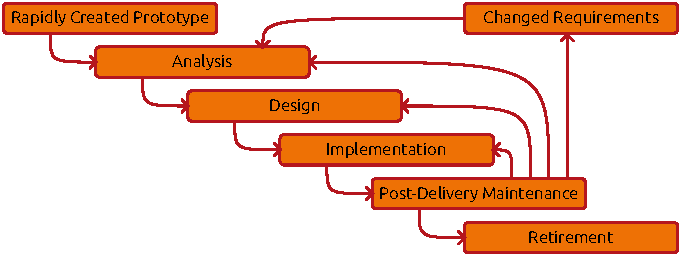
\includegraphics[width=0.8\linewidth]{\currentDir/rapid}%
\caption{The \pgls{RAD} model~\cite{S2007OOSE,GMTM2011DDLC,I2018SAH,N2024SEFDS}.}%
\label{fig:model:rad}%
\end{figure}%
%
\glsreset{RAD}\Pgls{RAD}, as illustrated in \cref{fig:model:rad}, lets the user try the application before it is delivered~\cite{S2007OOSE,GMTM2011DDLC,M1996RTWSS}.
If stakeholders can play around with a live system, then they can probably give much better feedback compared to a situation where they only work with specification documents.
Thus, a prototype is created and installed as soon as possible and made available to the user.
RAD-based projects tend to have a lower level of rejection when the application is placed into production.
The downside is that they are also likely to exhibit scope creep:
The stakeholders perceive modifying the application as easy and therefore are more likely to ask for more features.
The final goal of having a fully operational product may drift out of focus and the projects may overdraw budget and schedule.%
\FloatBarrier%
\endhsection%
%
\hsection{Databases Design Processes}%
\FloatBarrier%
%
\Pgls{db} systems differ from normal software applications.
On one hand, they usually are the foundation for \emph{several} software projects.
A student management \db\ for a university, for example, may offer the students to log in and join modules or view their grades.
It may also allow the administrative staff to create new modules and even manage the module structure of curricula.
It may furthermore handle the room planning for classes.
And it may even help to manage the important dates in the semester, such as times for exams, the schedule for students.
These things may be handled by different applications with different user interfaces.
But all of these applications would access the same \db\ backend.
Additionally, \dbs\ are long-living artifacts, which must be managed, maintained, and improved over many years.

As a result, a wide variety of design processes and life cycle management structures for \dbs\ have been developed.
They often are adaptations of different \pgls{SDLC} models and can offer different levels of detail to the project managers.

\begin{figure}%
\centering%
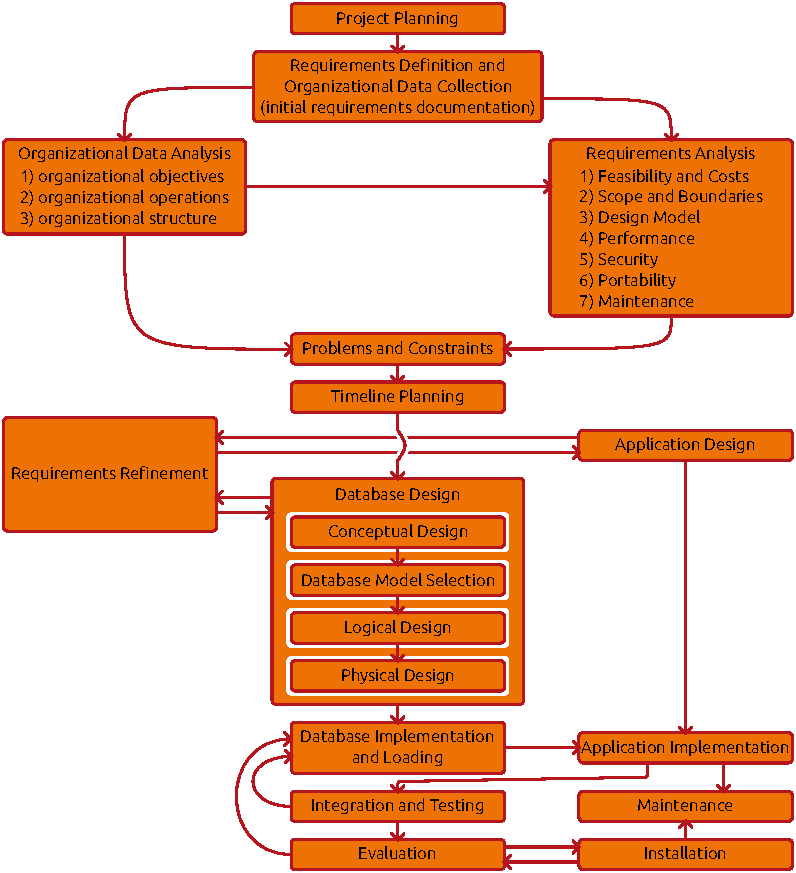
\includegraphics[width=0.8\linewidth]{\currentDir/gupta}%
\caption{The lifecycle model by~\citeauthor{GMTM2011DDLC}~\cite{GMTM2011DDLC}.}%
\label{fig:model:gupta}%
\end{figure}%
%
Personally, I like the comprehensive approach proposed by \citeauthor{GMTM2011DDLC}~\cite{GMTM2011DDLC} and illustrated in \cref{fig:model:gupta}.
It shows us all of the activities that a good \db~architect needs to consider.
In this model, the lifecycle begins with a planning stage.
Initially, there often are too many uncertainties to lay out a realistic timeline for the project.
Therefore, the goal of this first phase is to plan two activities:
(1)~the collection of the necessary information about the organizational processes that should be mirrored by the \db\ application and (2)~the requirements analysis.
The result of this phase is a plan document.

In the next stage, we collect all the data and information about the organization.
The developers and designers interact with all stakeholders in the project at all levels, from the intended users of the \db\ applications up to the management of the organization.
The documents and processes in the organization are explored, as well as the flow of data through the organization.
We check which systems and frameworks already exist, what input they require, what output the produce, who uses them and how and why.
Interviews and questionnaires can be used to gather more data.
The activities of personnel at all levels of the organization can directly be observed and documented.
The present needs and potential future expansions of the \db\ project are documented.
A software requirement specification is produced.

In the requirements analysis, we can now analyze the collected data to find out whether the project is feasible and to approximate the costs.
The goals of the project and the objectives of all proposed systems are specified.
The scope and boundaries (budget, equipment, available software) of the project are defined, as well as requirements regarding performance, security, portability, and maintenance.
All of these issues are very important for both the short term and long term success of the project.

As the result, potential problems and constraints that could arise later will be identified.
After the requirements collection and analyses are completed, a timeline for the rest of the project can be established.

\Pglspl{db} and the applications working on the data cannot be entirely separated.
The \db\ and the application(s) are therefore designed as two parallel strands of a project.
Both process update each other.
The first step of the \db\ design is to create a conceptual design, i.e., a high-level and technology-independent overview of the the \db.
The goal is to outline the big picture at an abstract level.
The model is based on the worldview and processes of the stakeholders.
This design can be visualized using \pglspl{ERD}~\cite{WF1995DHQDM,B1990CMERMO}.
It is common to \emph{not} just draw one single huge \pgls{ERD}, which would be overwhelming and hard to understand.
Instead, often, several smaller and easily readable \pglspl{ERD} are drawn with no more than ten or so entity types~\cite{WF1995DHQDM}.

Then, the \db\ model is chosen.
In the context of this book, our focus is on \pglspl{rdb}, where data is store in tables that can reference each other.
This may not always be the right choice.
For example, maybe we have to deal with images or video data, maybe we have to deal with results of simulations or computational experiments.
Then, other formats or \db\ paradigms may be more suitable.
Nevertheless, let us assume that \pglspl{rdb} are what we decide to use.
At this stage, we may also decide which \dbms\ to use.
This decision may be based on aspects such as costs, maintenance aspects, licenses, and available training.
In our book, we chose \postgresql, simply because it is a free (open source) and very mature \sql\ \dbms.

In the next step, the conceptual design is converted into a logical design.
This can mean to map the entity types from the \pglspl{ERD} in the conceptual models to tables and the relationships between them~\cite{SS2005EIDDDFDB:I,SS2005EIDDDFDB:CDDRAAML}.
Here, we may sometimes split one entity type from the \pglspl{ERD} into multiple tables or use different primary keys (e.g., sequential integers instead of a multi-part key constructed of strings\dots).
In other words, we map the conceptual model to the internal structures provided by the \dbms.
At this stage, we basically have an unoptimized design of the \db.

The logical design is then translated to a physical design.
This stage emphasizes the internal aspects of the database, e.g., the creation of access paths, indexes, the creation of partitions, and the implementation of business rules.
At this stage, we have a complete \db\ design, optimized for the planned operations.

The division in conceptual, logical, and physical design is not always defined like this.
Some approaches only distinguish the conceptual and the physical schema~\cite{G2011EW2ITDS:ITRD,V1999C5DMS:CI}.
In this case, the conceptual schema is also called logical schema and focuses on the specifications of the entity types and relations of the data.
The physical schema then comprises the two aspects that called physical and logical design above, i.e., the definition of tables, relations, and access paths.
From my perspective, which of the two approaches are chosen does not really matter.
Whether we have three-step or a two-step design method -- the important point is that we first model the data in an technological-independent and abstract way and later map this abstract model to a concrete design.

During the \db\ design phase, it is important to communicate and interact with the project stakeholders.
At this stage, the requirements may change again, which must be properly documented in the specifications.
While the \db\ is being designed, the user-facing applications are design in parallel.
Here, too, changes may be found necessary during discussions with the future users.

After the design phase, the database is implemented based on the physical design documents developed earlier.
The \db\ tables are created, populated with data, and constraints and queries are implemented.

Now that the \db\ exists, the application(s) can be implemented as well.
They are then integrated with the \db.
The system is tested.

Finally, the system is installed.
The users can now evaluate it.
The stakeholders can try the applications and judge its functionality and performance.
After the system has been accepted and enters the productive stage, the maintenance phase is entered.
The system is continuous upgraded, improved, and extended until it eventually reaches its end of life.

The method by \citeauthor{GMTM2011DDLC}~\cite{GMTM2011DDLC} sketched in \cref{fig:model:gupta} is a comprehensive approach for \db\ and software co-design in a large-scale project.
The main goal is to make \db\ projects more projectable.

Most lectures on \dbs\ focus more on the core of the development process, labeled \emph{Database Design} in \cref{fig:model:gupta} and often combine several of the framework activities such as installation and maintenance into one activity.

\begin{figure}%
\centering%
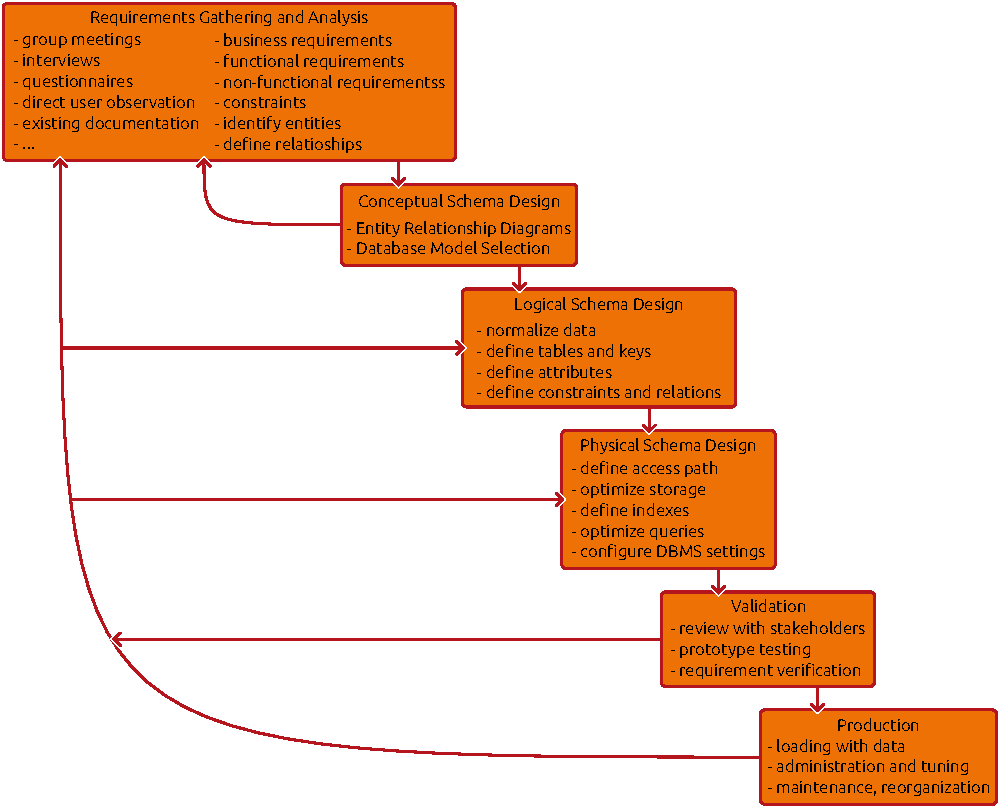
\includegraphics[width=0.96\linewidth]{\currentDir/ddlc}%
\caption{A simpler \db\ lifecycle model.}%
\label{fig:model:ddlc}%
\end{figure}%

In the context of this book, we, too, use a model with fewer steps.
It is illustrated in \cref{fig:model:ddlc} and combines ideas from several sources~\cite{SS2005EIDDDFDB:I,SS2005EIDDDFDB:CDDRAAML,D2022DN:DRA}.
Indeed, we will hinge the more comprehensive \db\ design example project discussed in this part of our book on this process.

This approach to the \db\ development life cycle begins with a phase of requirements gathering and analysis.
Then, the conceptual schema is designed:
The entities and their relationships are sketched with \pglspl{ERD}.
It makes sense to discuss this model with the stakeholders and, if any inconsistencies are discovered, to adapt the requirements specification.
In this step, we also choose the proper data model.

The entities in the conceptual model are then translated to fit to the data model in the logical schema design process.
In case of a relational data model (as used here), this means to create tables, define keys, attributes, and relations, and to normalize the data.
The physical schema is then the mapping of a logical schema to a concrete \dbms, including optimizations and efficient storage design.

Now a prototype can be developed and verified with the stakeholders.
Finally, the \db\ enters the production stage.
From here on, the focus is on maintenance, regular backups, fine-tuning, and the addition of features and adaptations to changed situations.
The last two stages can create feedback to the earlier stages, i.e., lead to changes in the physical or logical schemas as well as the requirements.

In the following, we will work our way step-by-step through this lifecycle.
By doing so, we will not just explore the different steps in more detail, but also discuss several important topics, such as \pglspl{ERD}, normalization, and $\sigma$\nobreakdashes-algebra based on a (more or less) realistic scenario.%
%
\FloatBarrier%
\endhsection%
%
\endhsection%
%
